%\pagestyle{empty}
%\cleardoublepage
%\pagestyle{fancy}
%\pagenumbering{arabic}

\chapter{Experimentos e Resultados}\label{cap5}
Neste capítulo detalhamos os experimentos realizados em quatro bases de dados. A primeira base de dados, coletada do vestibular da UFES, é utilizada para comparação de notas contínuas com o sistema proposto anteriormente por \citeonline{pissinati2014-master}. A base de dados de disciplinas da UFES e o \textit{Texas Dataset} foram análises do mapa de características como parte do \textit{software} na avaliação por classes antes e depois da redução de dimensionalidade. 

A última base de dados foi utilizada para testes de robustez do sistema. A base de dados do Prêmio de Avaliação Automática de Estudantes - ASAP (\textit{Automated Student Assessment Prize}) do \textit{Kaggle}, foge muito do padrão das demais correções do sistema pela quantidade de documentos e características. Assim, o \textit{dataset} foi aplicado na verificação da busca de padrões através da clusterização e do efeito da redução de dimensionalidade nos métodos de classificação em bases de dados maiores.

\section{Bases de Dados}\label{ss-databases}
Utilizamos nos testes quatro tipos de bases de dados de questões discursivas: do vestibular da UFES, de disciplinas ministradas por professores da UFES, da disciplina de Estrutura de Dados da Universidade do Norte do Texas (\textit{Texas Dataset}) e da competição da \textit{Hewllet Foundation} no \textit{Kaggle}. Cada base de dados é descrita à seguir.

\subsection{Base de Dados do Vestibular UFES} \label{vest-ufes-db}
Conjunto de atividades discursivas transcritas do vestibular de 2012 da Universidade Federal do Espírito Santo - UFES da prova de língua portuguesa. No total são 460 respostas para as cinco questões avaliadas por dois avaliadores, contendo 92 cada. Caso houvesse divergências de mais de 1 ponto entre as duas correções, um terceiro avaliador era acionado.

O enunciado das cinco atividades é apresentado na Seção \ref{sec-enunciados-vestufes} nos Apêndices.

\subsection{Base de Dados das Disciplinas UFES} \label{disciplinas-ufes-db}
Essa base de dados foi coletada de algumas disciplinas ministradas na Universidade Federal do Espírito Santo - UFES entre 2015 e 2016 através do Moodle do Laboratório Computação de Alto Desempenho - LCAD. Entre as disciplinas estão Metodologia e Técnicas de Pesquisa Científica, Filosofia e Tecnologia da Informação II. Totalizando 45 atividades, foram recebidas 1162 submissões com média 25,82 e desvio padrão de 13,54 respostas por atividade.

O diferencial dessa base de dados é a mudança de características nas respostas encontradas nas múltiplas disciplinas, professores e alunos. Observam-se alterações consideráveis quanto ao tamanho, número de grupos, critério avaliativo ou objetividade. 

\subsection{Base de dados da Universidade do Norte do Texas (Inglês)} \label{ds-cc-unt-db}
\textit{Dataset} coletado com alunos de Estrutura de Dados do curso de Ciência da Computação na Universidade do Norte do Texas. Resultado do trabalho realizado por \cite{mohler2011}, a base de dados, em sua segunda versão, constitui-se de dez atividades com sete questões e dois exames com dez questões cada. As provas foram avaliadas em intervalos de 0 a 10 e as atividades de 0 a 5 pontos. A avaliação foi feita por dois professores para as respostas de, em média, 30 alunos participantes. Após a avaliação foi extraída a média entre os dois corretores. No total, essa base de dados contém 630 respostas curtas e para cada atividade existe uma chave de resposta como o critério de correção do professor.

\subsection{Base de Dados do Concurso ASAG-SAS no \it{Kaggle} \bf{(Inglês)}}
\label{kaggle-db}
A competição de avaliação automática de questões discursivas curtas - \textit{ASAP - Automated Student Assessment Prize}, foi uma competição organizada no \textit{Kaggle}. O \textit{Kaggle} é uma plataforma de competições em mineração de dados que reúne tarefas complexas formadas por problemas reais enfrentados por grandes empresas. A sua comunidade era de 536 mil usuários registrados em 2016, que disputam prêmios e compartilham aprendizados em análise estatística e ciência de dados.

No \textit{Kaggle}, a organização \textit{Hewllet Foundation} patrocinou três competições. As três foram denominadas como as seguintes fases da ASAP:
\begin{itemize}
\item Fase 1:  Demonstração em respostas longas (redações); 
\item Fase 2:  Demonstração em respostas curtas (discursivas);
\item Fase 3:  Demonstração simbólica matemática/lógica (gráficos e diagramas).
\end{itemize}

A Avaliação Automática de Respostas Curtas (\textit{Automatic Short Answer Grader}) \textit{ASAG - SAS} premiou com um total de 100 mil dólares os cinco primeiros colocados. A base de dados de respostas curtas, contém dez questões de artes a ciências. Ao final do concurso, os dados disponíveis avaliados por dois professores totalizam 17043 itens com aproximadamente 1700 itens por atividade.


\section{Experimentos Realizados}
Para cada base de dados alguns experimentos foram realizados para efeito de comparação com os resultados da literatura. A base de dados do vestibular da UFES (Seção \ref{vest-ufes-db}), é utilizada para comparação desse trabalho com os experimentos realizados por \cite{pissinati2014-master} para avaliação em notas contínuas. 

O mapa de características e os sistemas de classificação foram testados em classes de nota de disciplinas universitárias. A base de dados coletada na UFES (Seção \ref{disciplinas-ufes-db}) foi construída durante os desenvolvimento do algoritmo de avaliação e do mapa de características. Para maior diversidade nos testes, esses também são realizados na base de dados de Estrutura de Dados da UNT (Seção \ref{ds-cc-unt-db}), em linguagem estrangeira. Essa última base de dados ainda conta com chaves de correção para parearmos as marcações formadas no mapa de características com as respostas aguardadas pelos professores.

Também em língua estrangeira, a base de dados do concurso ASAG-SAS no \textit{Kaggle}, é a com maior número de submissões e taxa de \textit{overllaping} testada. Essas duas informações são fundamentais para verificação da eficiência dos classificadores em situações de maior complexidade. Os resultados e as discussões envolvendo os métodos de classificação e a seleção de características são apresentados abaixo.

\subsection{Experimentos com o Vestibular da UFES}
O primeiro experimento realizado tem como objetivo analisar a equivalência do sistema desenvolvido com os resultados obtidos por \citeonline{pissinati2014-master}. Para isso, foi utilizada a mesma base de dados do vestibular da UFES com 460 respostas de alunos para cinco questões de Literatura/Português, avaliada por dois especialistas. No trabalho, o autor realizou sete experimentos para cada um dos avaliadores humanos do vestibular, também realizando uma comparação entre eles. O resultado dos trabalhos com base no Erro Médio Absoluto - MAE, tendo a divergência entre avaliadores como \textit{baseline}, é dado pelas Figuras \ref{exp-vest-mae1} e \ref{exp-vest-mae2} para o primeiro e segundo avaliador respectivamente.

\begin{figure}[ht]
\centering
\subfloat[Avaliador 1]{%
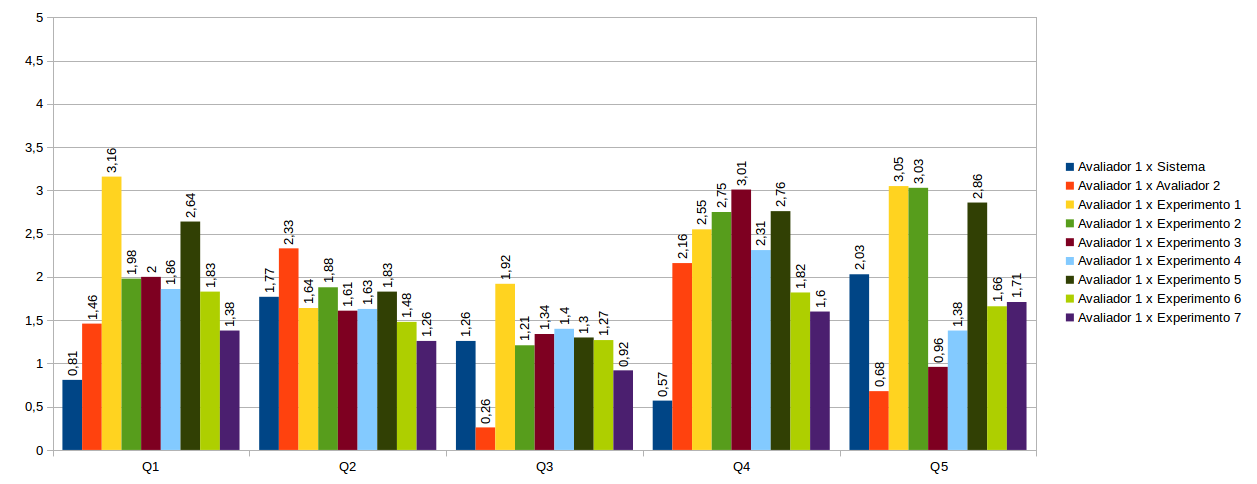
\includegraphics[width=\textwidth]{img/data_err1.png}%
\label{exp-vest-mae1}
}

\subfloat[Avaliador 2]{%
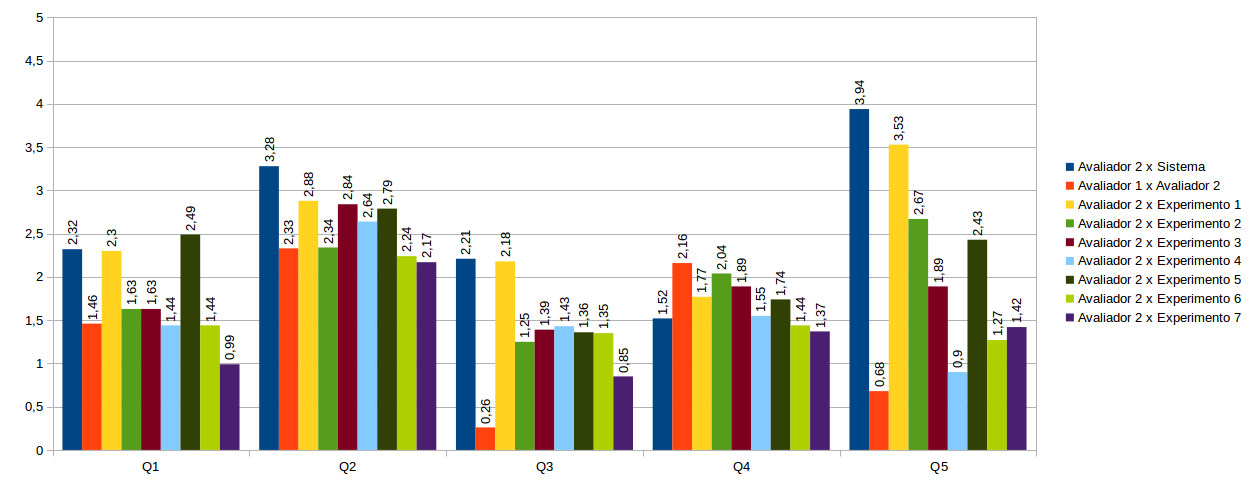
\includegraphics[width=\textwidth]{img/data_err2.png}%
\label{exp-vest-mae2}
}

\caption{Erro Médio Absoluto - MAE para os sete experimentos encontrados no trabalho tomado como referência, o sistema aqui apresentado e cada avaliador, utilizando como \textit{baseline} o erro entre os próprios especialistas.}
\end{figure}

Nas Figuras \ref{exp-vest-mae1} e \ref{exp-vest-mae2}, é possível visualizar a adequação do sistema com os avaliadores e com os melhores resultados apresentados nos sete experimentos. O único caso crítico observado, principalmente na adequação aos resultados do Avaliador 2, foi encontrado para questão 5. Nas demais, o sistema obtém resultados semelhantes aos melhores experimentos de \cite{pissinati2014-master}, sendo equiparável ao erro resultante dos dois avaliadores humanos. As Figuras \ref{exp-vest-dev1} e \ref{exp-vest-dev2} mostram o Desvio Padrão do Erro - SEM para os corretores humanos.

\begin{figure}[ht]
\centering
\subfloat[Avaliador 1]{%
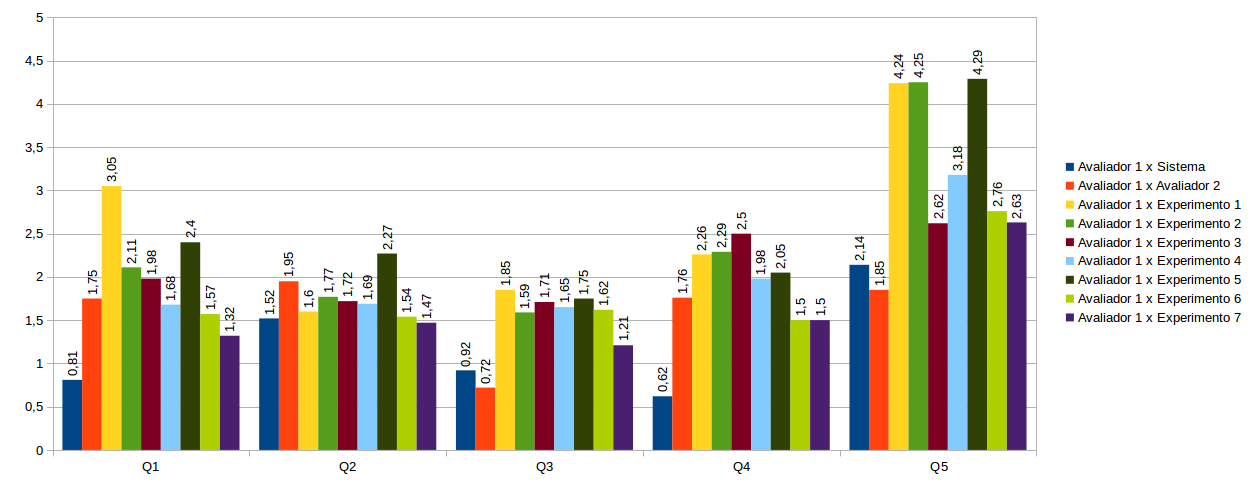
\includegraphics[width=\textwidth]{img/data_dev1.png}%
\label{exp-vest-dev1}
}

\subfloat[Avaliador 2]{%
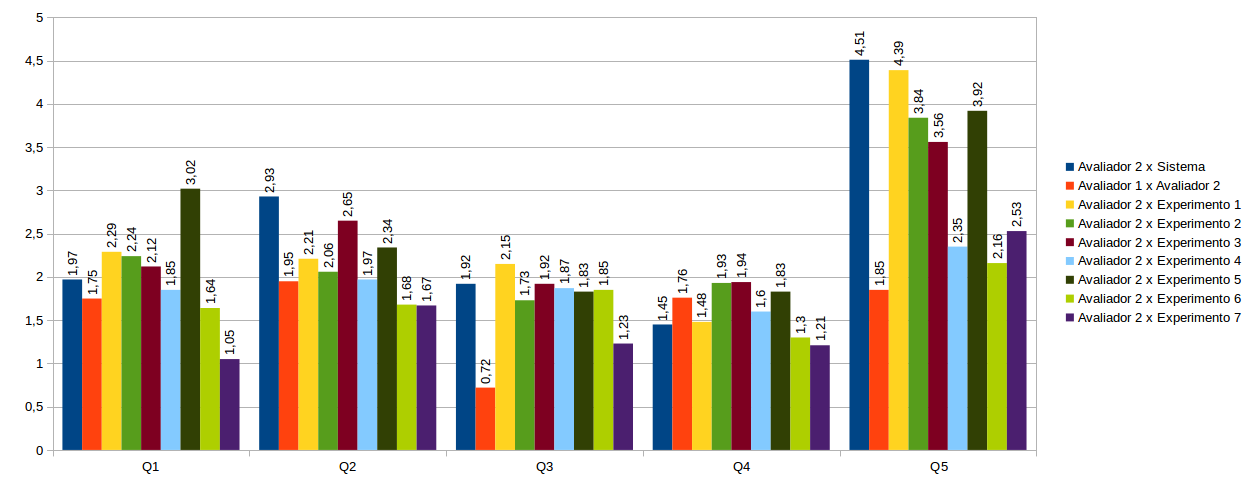
\includegraphics[width=\textwidth]{img/data_dev2.png}%
\label{exp-vest-dev2}
}
\caption{Desvio Padrão do Erro - SEM para os sete experimentos encontrados no trabalho tomado como referência, o sistema aqui apresentado e cada avaliador, utilizando como \textit{baseline} o erro entre os próprios especialistas.}
\end{figure}

Nas Imagens \ref{exp-vest-dev1} e \ref{exp-vest-dev2}, o desvio padrão médio de 1,202 pontos para o Avaliador 1 mostra que o sistema tem critérios de regulares de avaliação semelhantes a esse corretor, enquanto para o Avaliador 2 o desvio médio foi de 2,556 pontos. Quanto ao erro médio de 1,25 pontos para o primeiro avaliador e 2,32 pontos para o segundo avaliador mostramos que além de regulares temos bons modelos de avaliação. Os resultados são muito bons tendo em vista que o erro entre os dois humanos é, em média, 1,46 e os desvios 1,57 pontos.

Abaixo, vemos a descrição da atividade 5, para identificar o que possivelmente gerou os piores resultados:

\noindent\textit{``QUESTÃO 5: Com base nos elementos constitutivos do ato de comunicação, Roman Jakobson estabeleceu seis funções da linguagem (e a ênfase de cada uma delas): referencial (ênfase no assunto; no conteúdo), emotiva (ênfase no emissor; no sujeito), conativa (ênfase no receptor; no interlocutor), poética (ênfase na forma; na construção), metalinguística (ênfase no código; na autorreferência) e fática (ênfase no canal; no contato).}
\begin{itemize}
\item ``O navio negreiro'' - Castro Alves
\item ``7'' - Mário de Sá-Carneiro
\item ``Os arredores florem'' - Paulo Roberto Sodré
\end{itemize}
\textit{Escolha um dos textos da 4ª Questão indique e explique a ocorrência de uma dessas funções.''}

Nessa atividade, como vemos ao analisar o enunciado, esperam-se textos personalizados em cada resposta. Isso se deve a liberdade dada para cada estudante para escolher entre três textos e sete funções linguísticas, tornando a correção muito específica para cada resposta. A combinação de funções linguísticas com os textos disponíveis tornam a base de 92 textos transcritos pequena para a quantidade de padrões de resposta disponíveis. Possivelmente, o nível de erro apresentado é uma consequência dessa diversidade de padrões de resposta.

\subsection{Experimentos com as Disciplinas da UFES}
Após a validação do modelo básico por similaridade direta, essa segunda base de dados também em língua portuguesa, usa atividades de professores da UFES para a análise de aumento de similaridade e visualização da informação por classe de nota. O aumento de similaridade interna pode ser exemplificado através de duas tarefas (Figuras \ref{fig-redsim1-ufes} e \ref{fig-redsim2-ufes}). Nas figuras, estão as atividades \textit{TECII-5-169} e \textit{Filosofia-20-387} mostrando a similaridade interna de 0 à 1 para as classes de nota. A medida foi obtida pela média da similaridade interna por pares de documentos em cada nota antes e depois da seleção de características.

\begin{comment}
ANTES GA
0,0176	0,069	0,8571	0,9013	0,8571	0,8828	0,0168	0,056	0,8182	0,8947	0,8182	0,8182

DEPOIS GA
0,0292	0,069	0,8864	0,9429	0,8864	0,8866	0,0625	0,069	0,8	0,9286	0,8	0,8165
\end{comment}

\begin{figure}[!tbp]
  \subfloat[Média de similaridade interna para as classes da atividade TEC-II-5-169.]{
  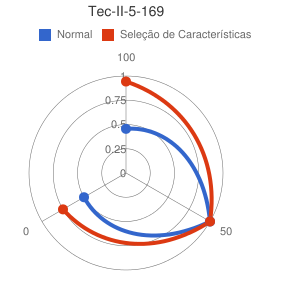
\includegraphics[width=0.45\linewidth]{img/red-ufes-moodle/image2.png}
  \label{fig-redsim1-ufes}}
  \hfill
  \subfloat[Média de  similaridade interna para as classes da atividade Filosofia-20-387.]{
  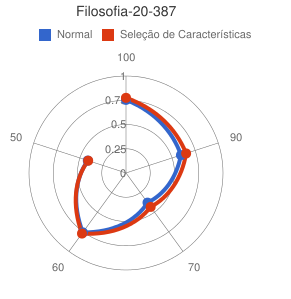
\includegraphics[width=0.45\textwidth]{img/red-ufes-moodle/image9.png}
  \label{fig-redsim2-ufes}
  }
  \caption{Similaridade interna por classe de nota em atividades de disciplinas da UFES antes e depois da seleção de características.}
\end{figure}

Como podemos observar nas Figuras \ref{fig-redsim1-ufes} e \ref{fig-redsim2-ufes}, existem ganhos superiores à 30\% de similaridade. Especificamente, se analisarmos os resultados apresentados nas Tabelas \ref{tab-exp-dis-ufes} e \ref{tab-exp-dis-ufes-features} do Apêndice, podemos ver que para as atividades apresentadas temos reduções de, respectivamente, 79,23\%, 54,05\% do total de características.

Para a atividade 1, \textit{Tec-II-5-169}, temos  42 características selecionadas para a classe 100, e apenas 1 para a classe 0. Para a classe 50, não tivemos redução por conta do grupos ser formado por apenas uma instância. Nesses casos, a análise de similaridade interna por pares não é aplicável e não ocorre redução. Assim, das 207 características distintas apenas 43 foram levadas em consideração. A similaridade interna nesse caso foi alta para a classe 100. Nessa classe a similaridade inicial de 0,4554 foi ampliada para 0,9431. Assim, os 42 termos retornados devem representar bem a resposta esperada pelo professor pois faz parte, praticamente, de todas as respostas avaliadas dessa forma.

Para a atividade 2, \textit{Filosofia-20-387}, apesar da redução para apenas 635 das 1382 iniciais, não observamos aumento da similaridade interna. Assim, as características foram identificadas para cada classe normalmente, mas o modelo de avaliação não torna a equivalência dos documentos exata para todas as respostas. Apesar de não ter sido ampliada pela seleção de características, a similaridade interna das amostras por classe se mantiveram em níveis altos. Para a classe 100, por exemplo, a similaridade interna foi de 0,7537 para 0,775. Normalmente, em casos onde ocorrem problemas na identificação das características relevantes os resultados são visivelmente ruins. Ao analisar a Tabela \ref{tab-exp-dis-ufes-classificacao} do Apêndice, encontramos para os dois classificadores utilizados resultados melhores para a atividade \textit{Tec-II-5-169}, com \textit{precision} e \textit{recall} de 100\%. Para a atividade \textit{Filosofia-20-387} com a questão ``Para o filósofo Kant, o que é ser livre?'', até por conta da abertura dada ao aluno, as métricas de classificação têm queda de \textit{accuracy} em 6\% para o K-NN e 8\% para o CBC.

Para as atividades dessa base de dados (Tabela \ref{tab-exp-dis-ufes-classificacao}), o classificador K-NN obteve resultados médios de \textit{precision} de 94,29\% e \textit{recall} de 88,64\%. Enquanto isso, para o CBC os resultados médios de \textit{precision} são de 92,86\% e de \textit{recall} 80,00\%.

\subsection{Experimentos com o \it{Texas Dataset}}
Outra base de dados testada, formada por respostas de questões da aula de Estrutura de Dados da Universidade do Norte do Texas. Para as atividades dessa base de dados, em geral as classificações foram melhores antes da seleção de características, que apresentou para o classificador KNN médias de \textit{precision} de 87,85\%, \textit{recall} de 81,80\% e \textit{accuracy} de 81,80\%. Com o CBC os resultados foram melhores, com \textit{precision} de 92,45\%, \textit{recall} de 87,50\% e \textit{accuracy} de 87,50\%. Esses resultados foram superiores aos valores apresentados por \cite{mohler2011}, com \textit{precision} de 85,00\% e \textit{recall} de 62,00\%.

Na classificação prevaleceram as classificações iniciais. Uma redução em \textit{precision} e \textit{recall} ocorreu para algumas atividades e são associadas à perda de informação da redução de dimensionalidade como apresenta a Tabela \ref{tab-exp-mohler-features} do Apêndice. Isso ocorre quando o mapa de características não encontra boa intercessão por classe de nota. Das 86 atividades, para o classificador K-NN 27 tiveram uma mudança positiva em \textit{precision} enquanto em 34 a mudança foi negativa. Nas demais 25 atividades não tiveram alterações maiores de 0,1\%. Porém, o classificador CBC apresentou maiores problemas quanto a isso. Após a redução, em 56 atividades tiveram queda de \textit{precision} enquanto 18 apresentaram melhoria. Nas outras 12 atividades não ocorreram alterações significativas. Apesar disso, o sistema não influencia negativamente na construção dos mapas de características. 

Em geral, são bons os resultados médios de \textit{precision} e \textit{recall} mesmo após a redução de dimensionalidade com, respectivamente, 86,3\% e 74,4\% para o KNN 82,3\% e 73,3\% para o CBC. As métricas de classificação para os dois algoritmos antes e depois da seleção de características em cada atividade também estão disponíveis na Tabela \ref{tab-exp-mohler-classificacao} do Apêndice.

\begin{comment}
0,0305	0,07	0,818	0,8785	0,818	0,819	0,023	0,049	0,875	0,9245	0,875	0,883

0,035	0,0795	0,774	0,863	0,776	0,7785	0,0755	0,13	0,732	0,826	0,733	0,7015

\end{comment}

\subsection{Experimentos com Dados do \it{Kaggle}}
A base de dados do \textit{Kaggle} foi utilizada de forma distinta da perspectiva da competição. Apenas são utilizados os dados de treinamento para aquisição de informações por \textit{clustering}. Os demais dados não selecionados pela aquisição de padrões de correção formaram o conjunto de teste da classificação. A única alteração no processo dos demais experimentos foi o aumento do número inicial dos testes de melhor \textit{clustering}. O início da busca foi de 3 para em 30 \textit{clusters}, visando contornar as altas taxas de \textit{overlapping} dado o \textit{silhouette score} negativo em boa parte dos agrupamentos. Além disso, essa mudança causa aumento no percentual de treino para alcançar números significativos. Os dados de treinamento e o número de \textit{clusters} para cada atividade é apresentada na Tabela \ref{tab-kaggle-clustering}.

\begin{table}
\centering
\resizebox{\textwidth}{!}{%
\begin{tabular}{l|c c c c c c c c c c}
\hline
\textit{Dataset} KAGGLE &  1 &  2 & 3 & 4 &  5 & 6 & 7 & 8 & 9 & 10\\ \hline
Nº Grupos & 38 & 46 & 30 & 30 & 41 & 59 & 39 & 56 & 44 & 45 \\
Treino (em \%) & 12,56 & 19,25 & 8,99 & 9,90 & 12,48 & 16,92 & 12,12 & 16,51 & 13,40 & 15,24 \\
Treino (em respostas) & 210 & 246 & 170 & 172 & 224 & 304 & 218 & 297 & 241 & 250 \\
Total (em respostas) & 1672 & 1278 & 1891 & 1738 & 1795 & 1797 & 1799 & 1799 & 1798 & 1640 \\
\hline
\hline
\end{tabular}}
\caption{Informações de treinamento da base de dados após particionamento durante a análise de distribuição na etapa de \textit{clustering}.}
\label{tab-kaggle-clustering}

\end{table}

Podemos ver através da Tabela \ref{tab-kaggle-clustering} que temos um esforço muito baixo de correção apesar do aumento do número mínimo de \textit{clusters}. Devemos observar a representatividade desse treino conforme os resultados de classificação. Os detalhes da avaliação segundo \textit{precision} e \textit{recall} estão disponíveis na Tabela \ref{tab-exp-kaggle-classificacao}, observando o impacto da seleção de características e a compatibilidade com a avaliação de cada avaliador.
 
\begin{table}[ht]
\resizebox{\textwidth}{!}{%
\begin{tabular}{l|c|cc|cc|cc|cc|}
& & \multicolumn{4}{|c|}{Antes da Seleção de Características} & \multicolumn{4}{|c|}{Depois da Seleção de Características}  \\
& & \multicolumn{2}{|c|}{KNN} & \multicolumn{2}{|c}{CBC} & \multicolumn{2}{|c|}{KNN} & \multicolumn{2}{|c|}{CBC} \\
\textit{Dataset} & Avaliador & \textit{Precision} & \textit{Recall} & \textit{Precision} & \textit{Recall} & \textit{Precision} & \textit{Recall} & \textit{Precision} & \textit{Recall} \\ \hline

\input{tables/kaggle-experimentos.csv}

\hline
\end{tabular}}
\caption{Avaliação da classificação para cada atividade da base de dados conforme 6 métricas e dois classificadores antes e depois da seleção de características.}
\label{tab-exp-kaggle-classificacao}

\end{table}

A Tabela \ref{tab-exp-kaggle-classificacao} apresenta a compatibilidade da correção do sistema para os dois avaliadores. Podemos, com base nas métricas aferir que algumas atividades têm problemas de representatividade pois \textit{precision} é muito próximo aos 50\%. Nos casos de \textit{precision} baixa, a extração de informações \textit{intra-cluster} provavelmente não é suficientemente abrangente, o que é esperado com um treinamentos em torno de 10\% dos documentos. O que não ocorre quando mais exemplos são utilizados para treinamento. Uma análise refinada desses grandes \textit{clusters} deverá ser realizada para uma subdivisão ou a aquisição de uma quantidade maior de treino buscando dados mais representativos. 

Para a classificação dos demais itens é relevante salientar o seu bom desempenho em sete dos dez \textit{datasets}. Os classificadores alcançam \textit{precision} médio de 76,51\% para o primeiro avaliador e 76,00\% para o segundo, com destaque para as atividades 4, 5 e 6 que apresentaram valores acima dos 90\%. Sabendo do grande número de submissões se comparada com as demais bases de dados, a adequação ao método avaliativo de ambos corretores mostra a eficácia do \textit{software} e seu baixo de esforço de correção necessário. Sendo que, a base de dados particionada foi disponibilizada inteiramente para treinamento dos algoritmos participantes da competição, ao qual usamos menos de 20\% dos itens para correção.

\begin{comment}
KAGGLE 1 & 0.8940 & 0.8941 \\
KAGGLE 2 & 0.8533 & 0.8537 \\
KAGGLE 3 & 0.7608 & 0.7609 \\
KAGGLE 4 & 0.7843 & 0.7819 \\
KAGGLE 5 & 0.9660 & 0.9654 \\
KAGGLE 6 & 0.9695 & 0.9694 \\
KAGGLE 7 & 0.9592 & 0.9594 \\
KAGGLE 8 & 0.8393 & 0.8399 \\
KAGGLE 9 & 0.8083 & 0.8087 \\
KAGGLE 10 & 0.8857 & 0.8847 \\
\end{comment}

\subsection{Experimentos com Mapa de Características} \label{exp-mapas}
O mapa de características, como apresentado no Capítulo \ref{cap4}, é uma forma de visualização dos resultados segundo a representatividade dos termos. As marcações propostas são automaticamente relacionadas conforme a avaliação do professor e o modelo de avaliação do \textit{software}. O resultado das marcações são termos destacados pela correlação com uma nota (com a cor específica) ou neutra (com a cor preta), esse último caso ocorre em baixa ou nula correlação com a avaliação. Para o mapa de características os demais termos não marcados não fazem parte do conteúdo essencial de nenhuma classe de nota.

Para as atividades do \textit{Texas Dataset} temos, além da avaliação, respostas aguardadas apresentados pelos corretores. Por exemplo, na atividade \textit{1.5} apresentada na Figura \ref{UNT-15}, os alunos responderam a seguinte pergunta: ``\textit{what is a variable?}''. Nas respostas vemos marcações que relacionam quatro notas distintas com os termos. Essas marcações variam em 10 tons de coloração de 0 equivalente à neutro até 9 com alta correlação à nota. Os termos não marcados são desconsiderados pelo sistema. As alterações de tonalidade são dispostas em até 6 cores vinculadas a uma nota específica.


\begin{figure}[h!]
\centering
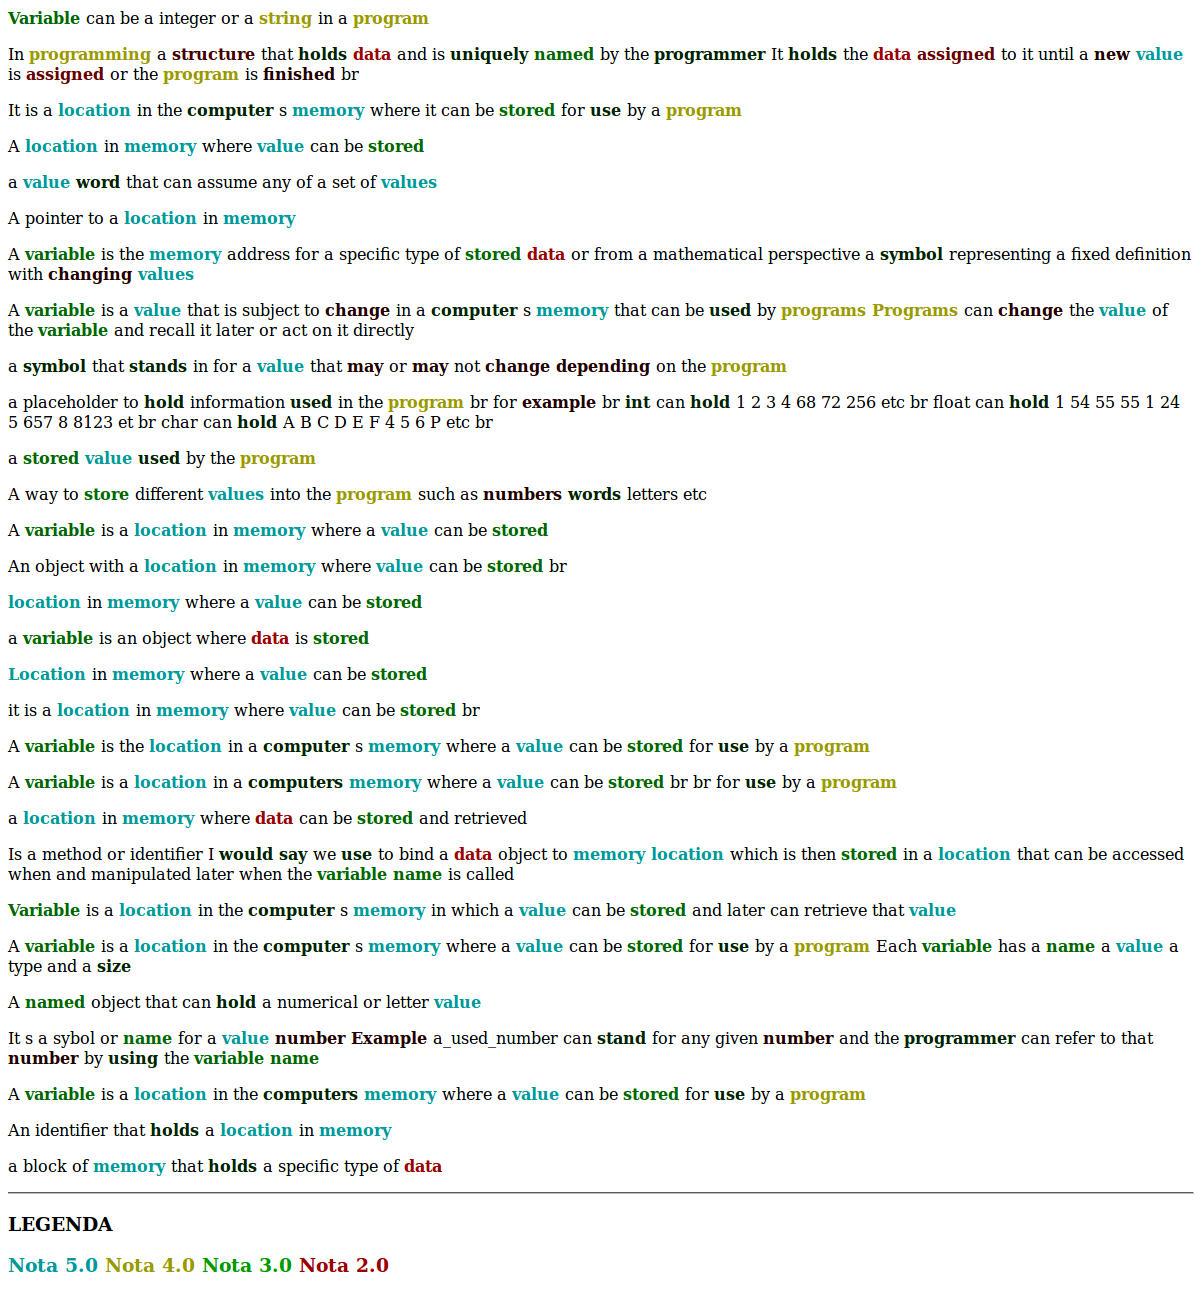
\includegraphics[width=\textwidth]{img/UNT-1-5.png}
\caption{Mapa de características de todos os alunos para a atividade \textit{DS CC UNT 1-5}.}
\label{UNT-15}
\end{figure}

Na Figura \ref{UNT-15} podemos ver que as palavras \textit{location}, \textit{memory} e \textit{value} são fortemente ligadas com a nota máxima \textit{5,0} em azul. Enquanto isso \textit{program} e \textit{string} pertencem ao grupo de nota \textit{4,0} em amarelo, \textit{variable} \textit{name} e \textit{stored} ao de nota \textit{3,0} em verde e \textit{data} e \textit{assigned} remetem à nota \textit{2,0} em vermelho. Palavras pouco correlacionadas como \textit{symbol}, \textit{example}, \textit{computers} e \textit{programmer} são consideradas neutras. Porém, se compararmos as marcações com a resposta esperada apresentada pelo professor ``\textit{a location in memory that can store a value}'', temos as principais palavras diretamente relacionadas ao critério de correção.

Apesar disso, para apresentar a influência da avaliação na ponderação dos termos podemos analisar uma questão de nota única como a \textit{9.7}, marcada em vermelho. A pregunta apresentada aos alunos foi ``\textit{what data structure is more appropriate for scheduling printing jobs at a printer, a stack or a queue?}''. A resposta aguardada para essa pergunta é ``\textit{queue}'' e pode ser vista em todos os documentos da Figura \ref{UNT-97}.

\begin{figure}[h!]
\centering
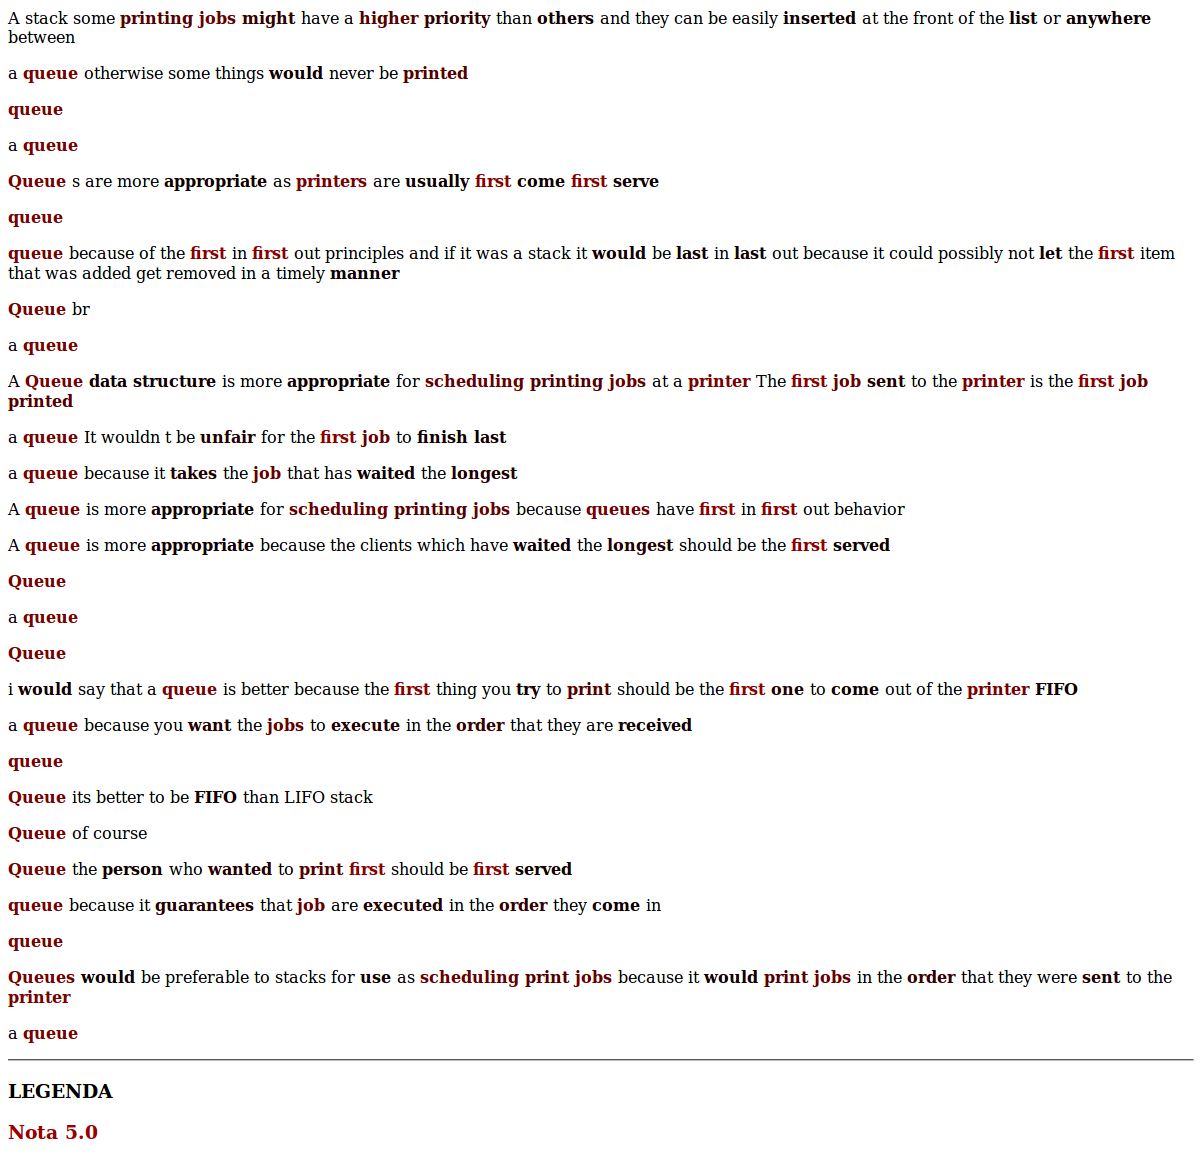
\includegraphics[width=\textwidth]{img/UNT-9-7.png}
\caption{Mapa de características de todos os alunos para a atividade \textit{DS CC UNT 9-7}.}
\label{UNT-97}
\end{figure}

Através da Figura \ref{UNT-97} podemos descrever a função de seleção de forma simplificada. O fato da atividade toda ser avaliada com a nota 5 e todas as respostas conterem \textit{queue} a correlacionam fortemente com a nota. As demais palavras marcadas, são realçadas pelo sistema apenas por aparecerem com certa frequência, mesmo não sendo o núcleo da resposta. Isso ocorre por exemplo com \textit{appropriate}, \textit{first}, \textit{job}, \textit{printer}. Os termos neutros marcados em negrito não são tão representativos à ponto de serem relacionados com uma nota. Na atividade \textit{2-6}, por exemplo, ocorrem avaliações não polarizadas (neutras) para a pergunta ``\textit{what is the difference between a function prototype and a function definition?}''. Os documentos dessa questão são apresentados na Figura \ref{UNT-26}.

\begin{figure}[h!]
\centering
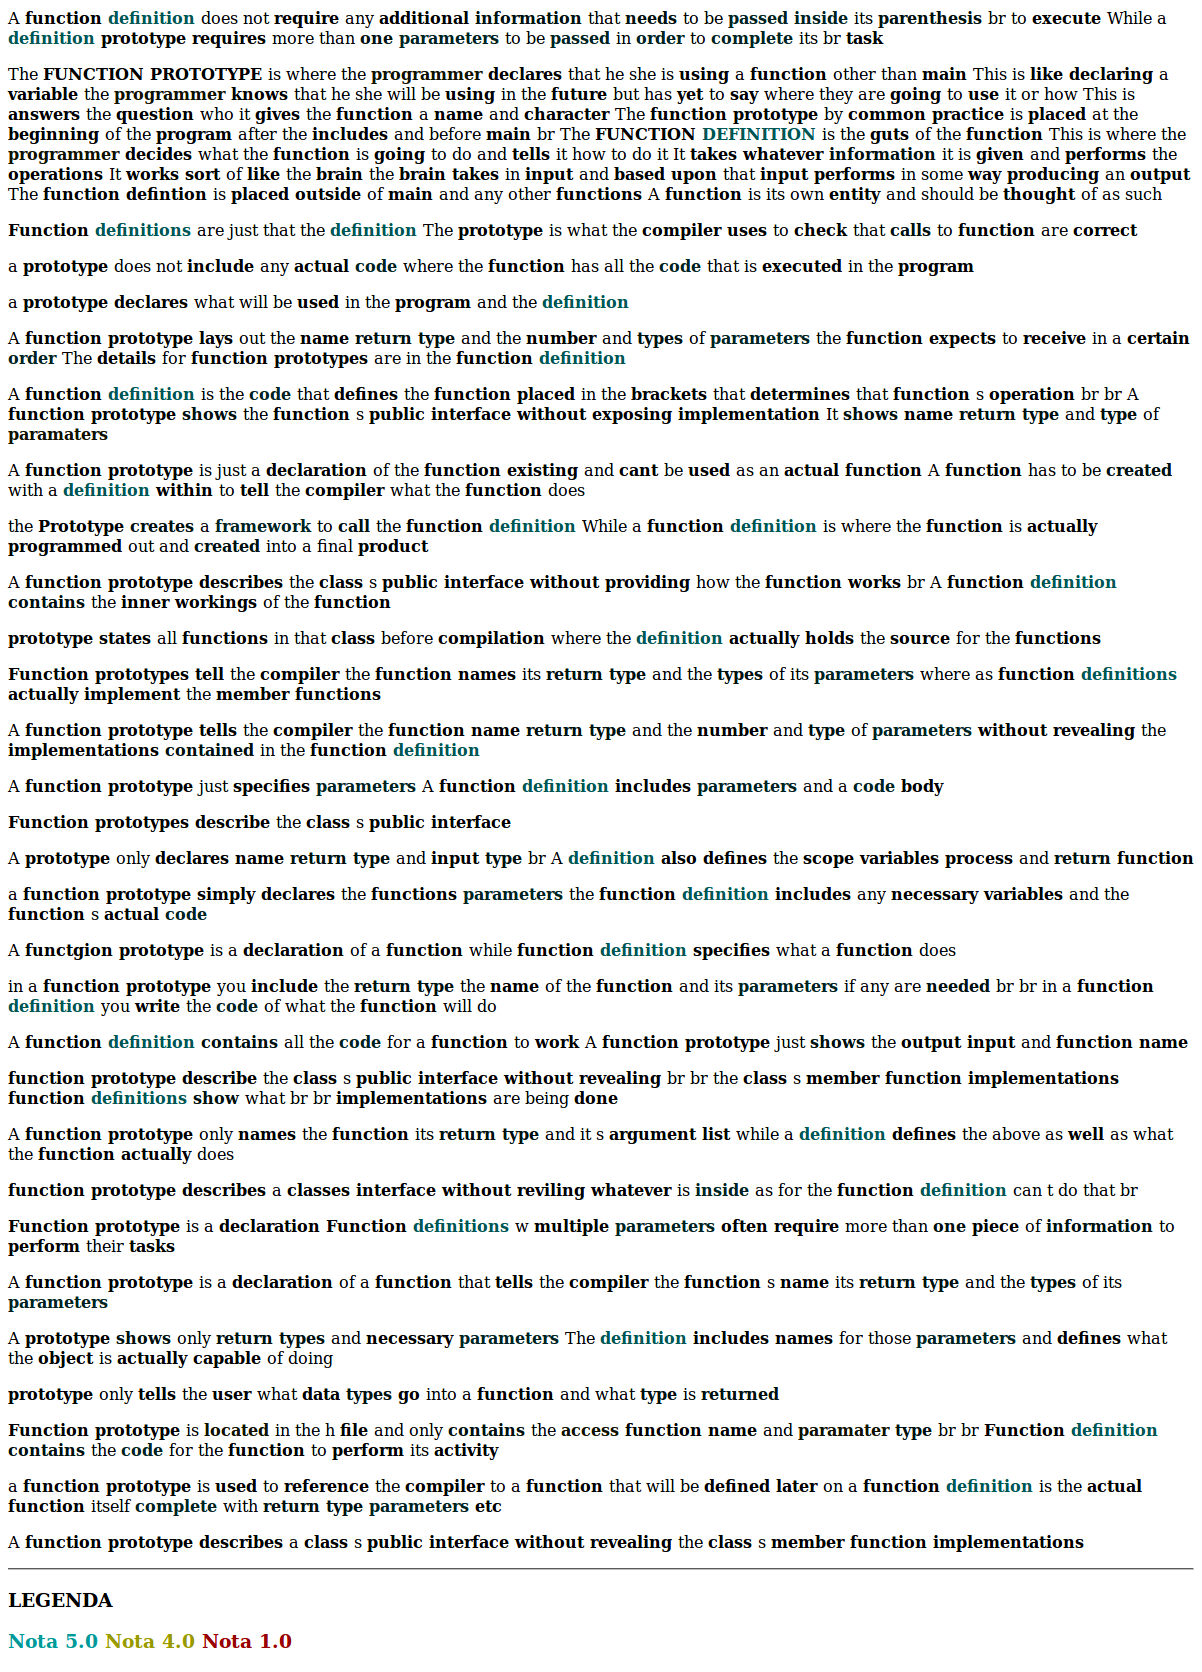
\includegraphics[width=\textwidth]{img/UNT-2-6.png}
\caption{Mapa de características de todos os alunos para a atividade \textit{DS CC UNT 2-6}.}
\label{UNT-26}
\end{figure}

Podemos analisar a Figura \ref{UNT-26} paralelamente com a chave de correção do professor para verificar os possíveis motivos da quantidade de marcações neutras. A resposta aguardada era ``\textit{a function prototype includes the function signature, i.e., the name of the function, the return type, and the parameters' type. The function definition includes the actual body of the function}''. Pelos documentos da figura e a chave de correção vemos que a enumeração de partes de uma função era a essência da resposta. Porém, ao contrário do aguardado, não temos intercessão observável exceto em \textit{function prototype} e \textit{function definition}. Tais trechos são encontrados nas respostas das três notas disponíveis (\textit{5,0 3,0} e \textit{1,0}). Assim, o processo de avaliação foi criterioso quanto a diferenciação entre as funções, independentemente do aspecto elencado. Isso confunde o algoritmo pela ausência de termos semelhantes por classes de nota ao coexistirem várias respostas possíveis.

Apesar da ocorrência de ``questões neutras'' quanto ao conteúdo podemos ver em mais um exemplo de questão através da capacidade de interpretação das marcações. Para o enunciado ``\textit{what is the difference between a circular linked list and a basic linked list?}'', temos respostas bem consistentes. A Figura \ref{UNT-75} apresenta as submissões dos alunos avaliadas em duas notas \textit{5,0} e \textit{2,0} pelo professor.


\begin{figure}[h!]
\centering
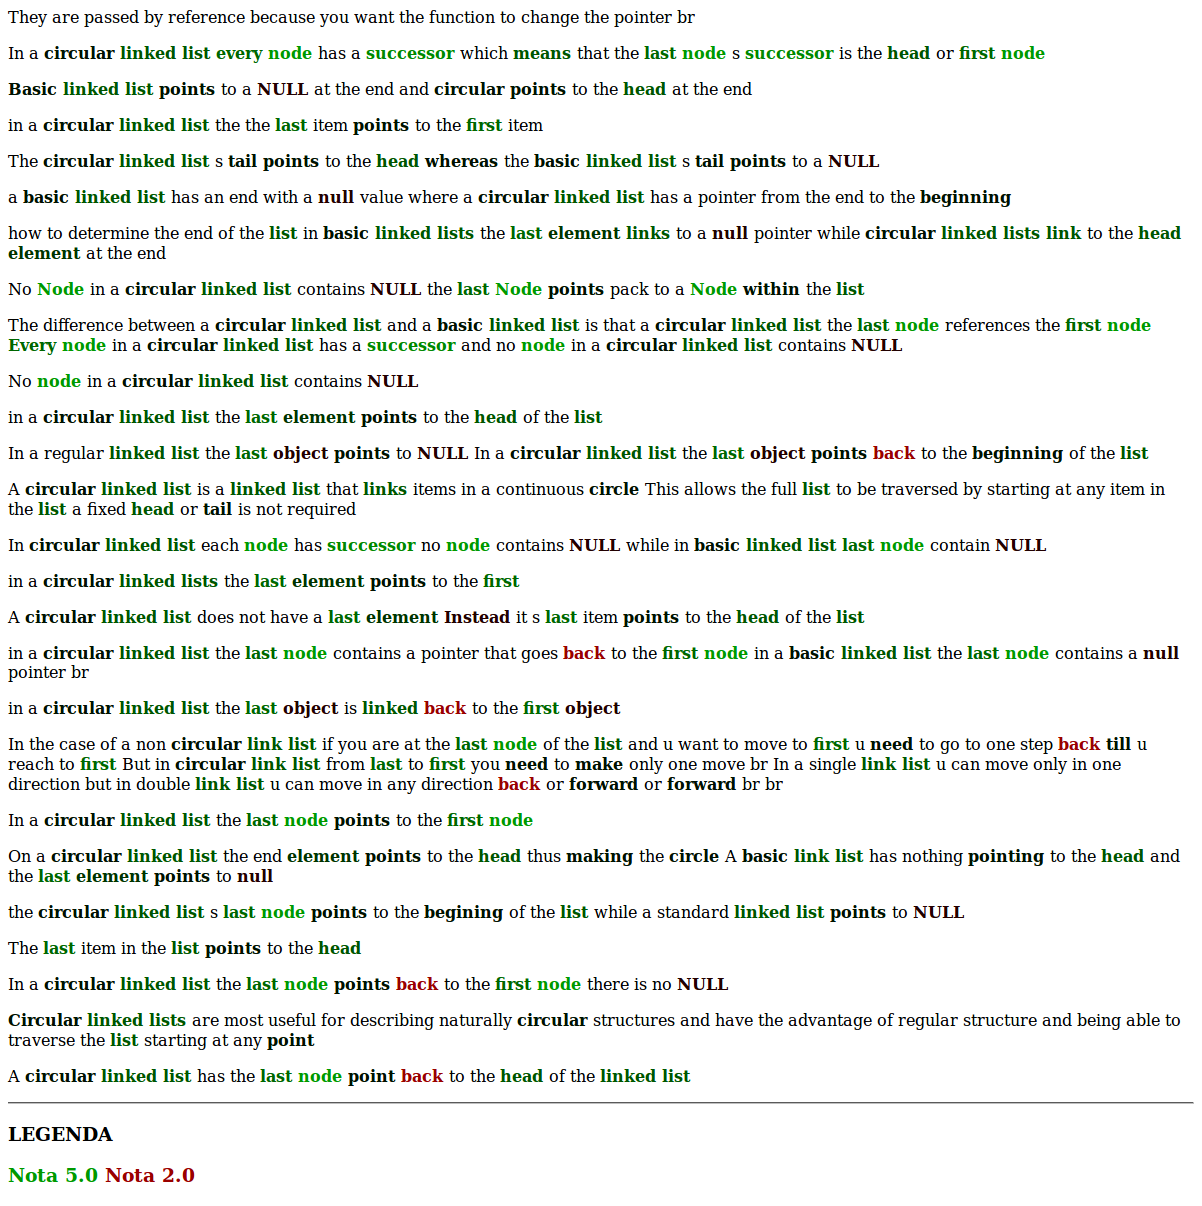
\includegraphics[width=\textwidth]{img/UNT-7-5.png}
\caption{Mapa de características de todos os alunos para a atividade \textit{DS CC UNT 7-5}.}
\label{UNT-75}
\end{figure}

Podemos ver na Figura \ref{UNT-75} que para uma lista encadeada (\textit{linked list}) em vez de nulo (\textit{null}) a referência do ultimo nó (\textit{last node}) deve ser para o primeiro nó (\textit{first node} ou \textit{head}). E exatamente essa resposta era aguardada pelo professor: ``\textit{the last element in a circular linked list points to the head of the list}''. A palavra \textit{back} atribuiu fator negativo de avaliação pois em uma estrutura de dados circular a sequência do último item é o inicial. Esse termo quando utilizado para uma estrutura de dados passa a ideia de retorno por todos os itens, ao contrário do que efetua o código, direcionando-o por referência.

As atividades em português da base de dados de disciplinas da UFES tiveram resultados semelhantes. Podemos, ao observar a Figura \ref{Ufes170}, ver comportamentos da marcação equivalente ao da Figura \ref{UNT-75}. Tanto para a atividade \textit{DS CC UNT 7-5} quanto para a \textit{Tec-II-5-170} um detalhe foi crucial para diferenciar dois níveis de nota. Para essa segunda, existe maior esforço do sistema no reconhecimento das características para a questão ``Cite algumas linguagens para o lado do servidor''. Isso ocorre por conta da liberdade dos alunos para escolher qualquer linguagem de programação executadas no servidor.


\begin{figure}
\centering
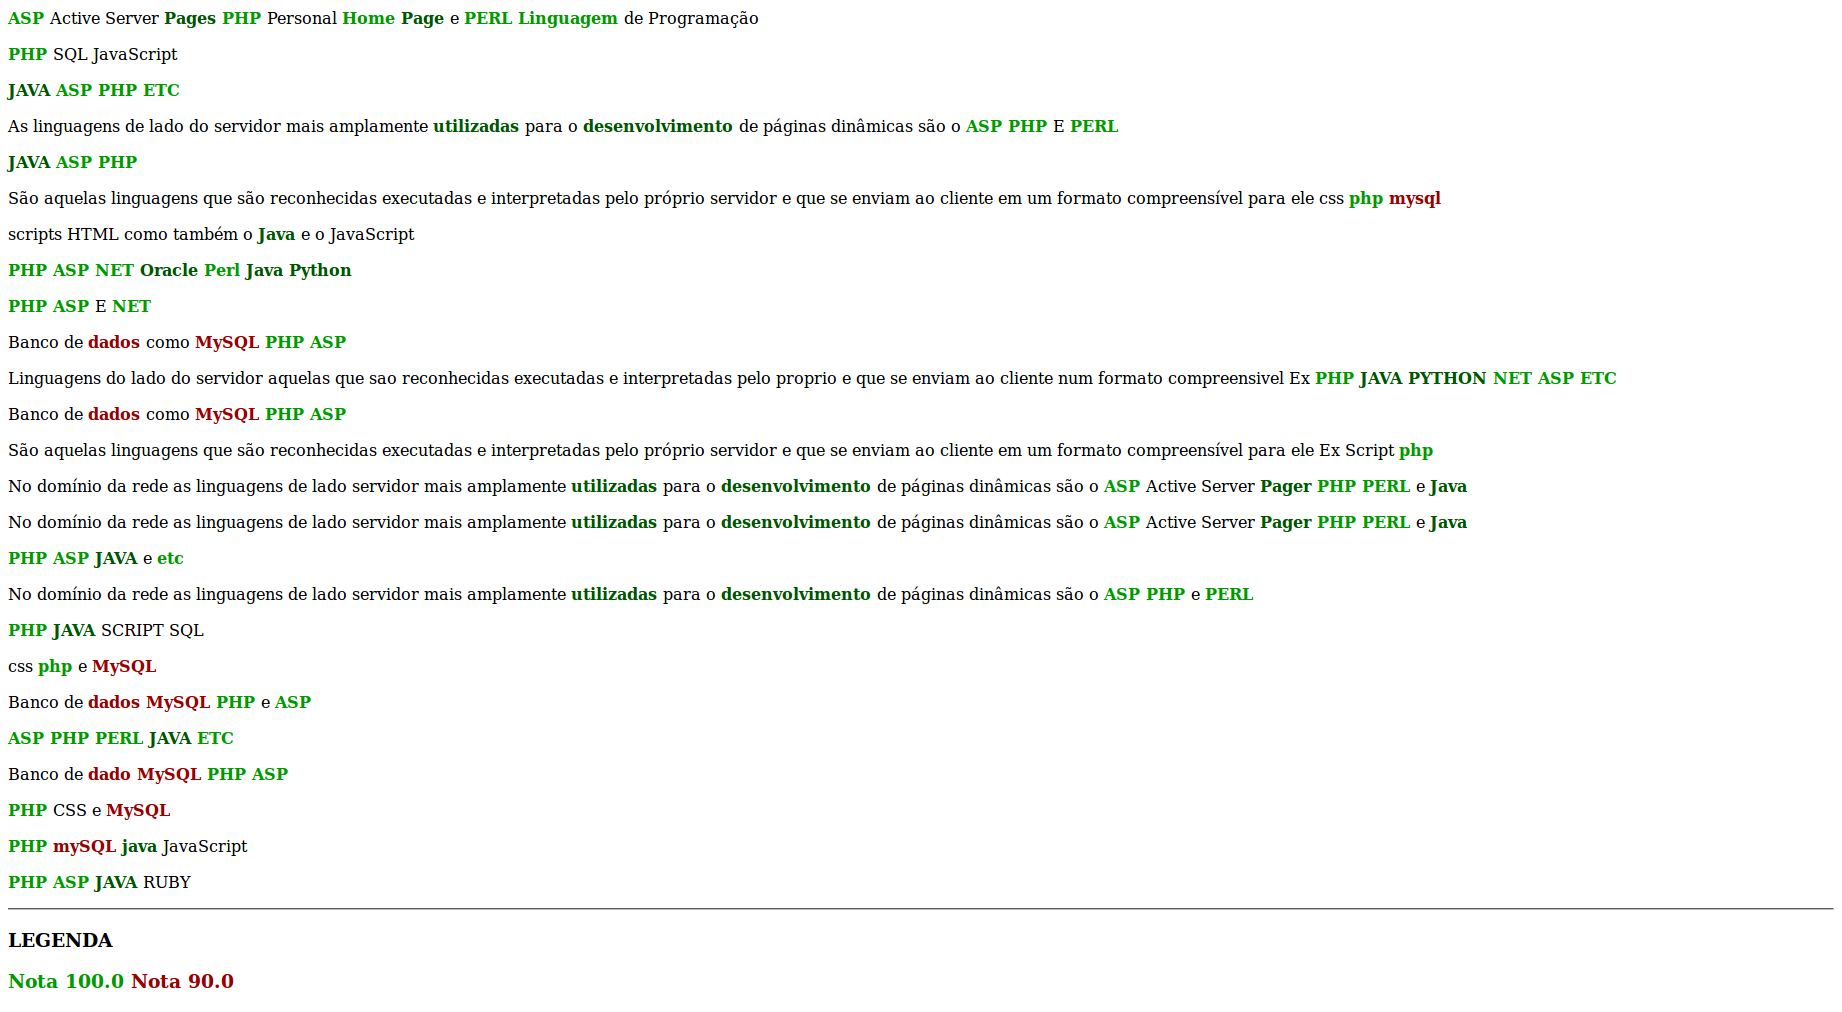
\includegraphics[angle=90, width=0.75\textwidth]{img/Ufes170.png}
%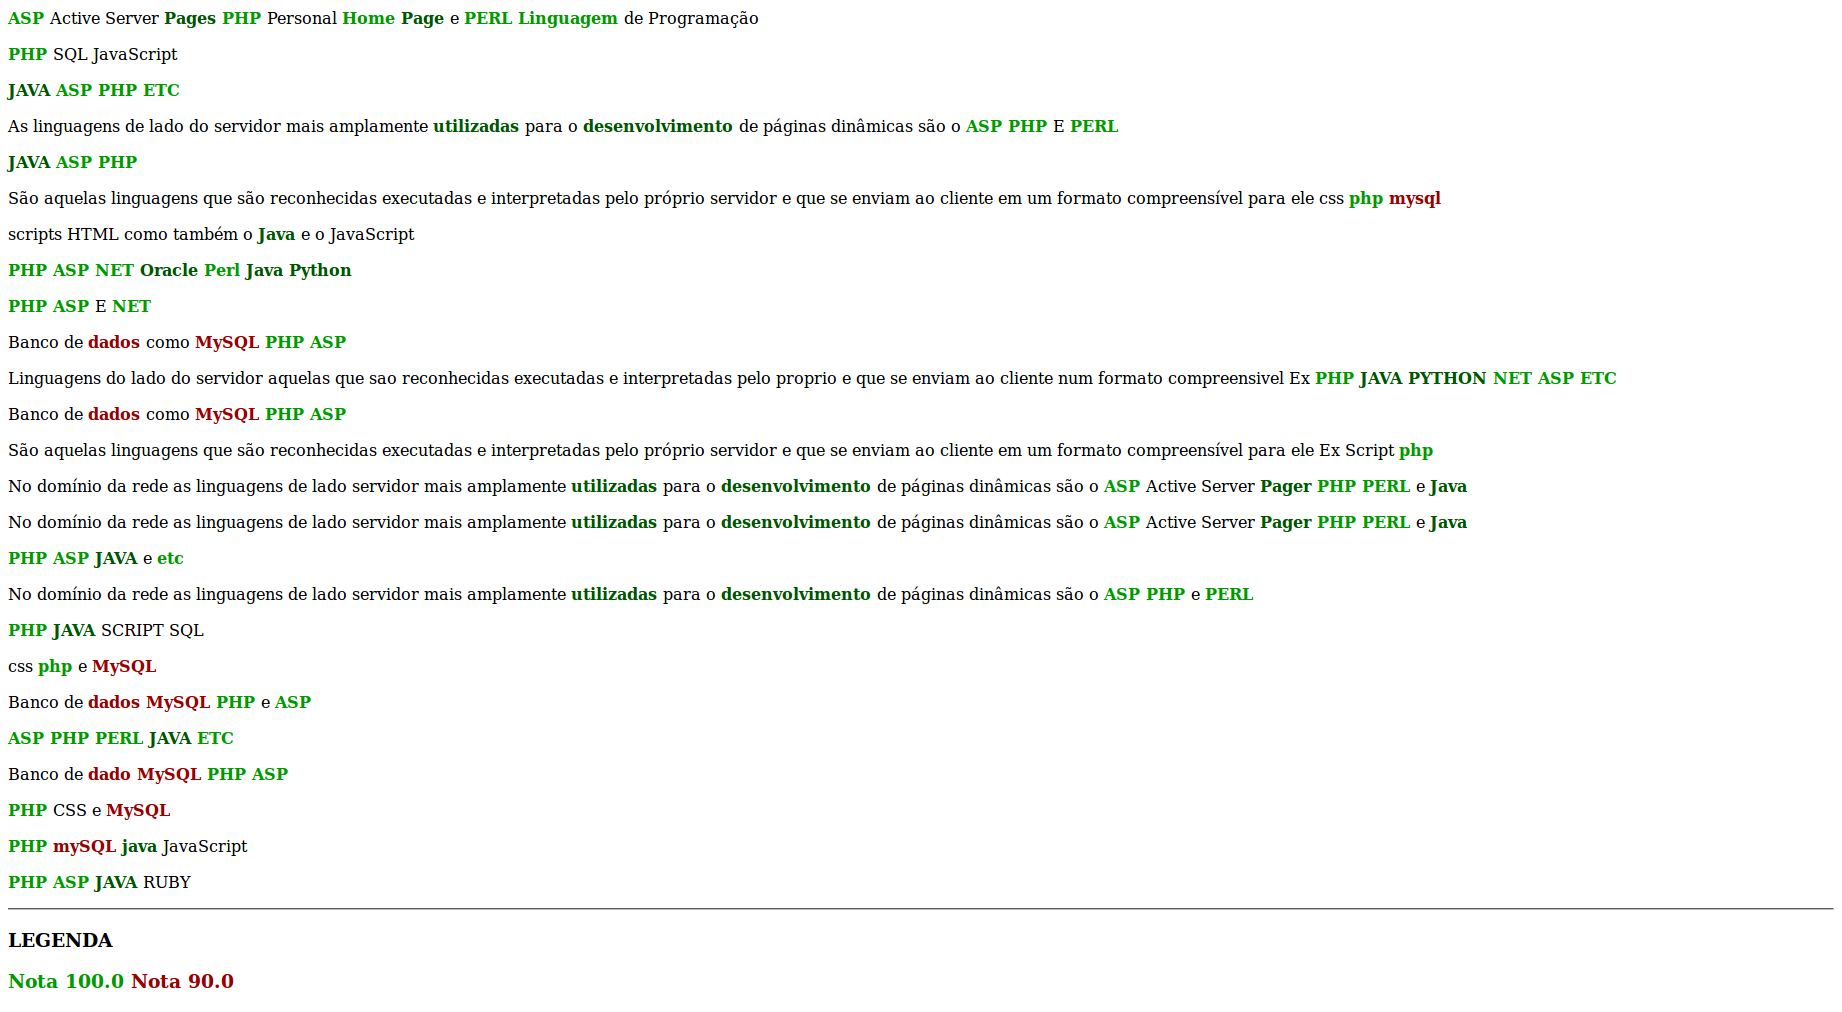
\includegraphics[width=\textwidth]{img/Ufes170.png}
\caption{Mapa de características de todos os alunos para a atividade \textit{Tec-II-5-170}.}
\label{Ufes170}
\end{figure}

Nesse caso, a Figura \ref{Ufes170} deixa bem explícito o decrécimo da nota associado ao termo ``mysql''. Obviamente, por ser um sistema gerenciador de banco de dados e não uma linguagem de programação, como aguardado nas respostas, era avaliado negativamente pelo professor. Nas marcações, esse termo é associado à classe 90.0 enquanto as demais ``ASP'', ``PHP'', ``.Net'', ``Python'' ``Pearl'' e ``Java'' remetem à nota 100.0.

\section{Discussão}
Nas atividades do Vest-UFES a comparação do sistema com os experimentos de pré-processamento de \cite{pissinati2014-master} temos resultados equivalentes. O sistema em todas as atividades adquire métodos avaliativos semelhantes ao Avaliador 1, tendo como \textit{baseline} o erro entre especialistas. O autor, contudo, alcança resultados próximos aos dois avaliadores apenas após sete experimentos cumulativos. Nos modelos de avaliação, ambos os sistemas superam a correção humana nas métricas avaliadas, sendo que a análise das diferenças deve ser um fator descritivo quanto ao erro. Erros de um grau de nota, ou seja, apenas um nível de classe de diferença geralmente são considerados comuns até entre especialistas \cite{bazelato2013}. O baixo desvio padrão indica a ocorrência desse tipo de erro.

A comparação com os experimentos do autor, com o intuito de validar o modelo de avaliação, apresenta que o sistema aqui proposto tem boa atuação até mesmo em notas contínuas. Além disso, atividades de língua portuguesa, quando voltadas para a análise textual, induzem os estudantes a interpretações distintas. Assim, com exceção  da questão 5 para o segundo avaliador, o sistema tem grande qualidade resultando um baixo nível de erro.

Para as atividades das disciplinas da UFES temos como foco a avaliação por notas discretas (classes). Essa base de dados colaborou com as formas de análise de similaridade e estudo de distribuição das respostas. Com o trabalho em classes de nota, podemos observar a classificação do especialista de forma a buscar critérios específicos. Com a redução de ruídos e a sumarização através do algoritmo genético, grupos muito similares melhoraram a classificação. Enquanto isso, nas situações onde ocorreu certa dificuldade de extração dos termos ideais indicaram que o critério de correção foi além do conteúdo analisado pelo sistema ou os termos não foram correlacionados à nota tal como deveriam.

Nos casos onde algum problema referencial ao texto foi encontrado os resumos dos documentos após seleção de características não foram tão representativos. Por exemplo, se na etapa de correção o professor for indiferente quanto ao conteúdo do texto são gerados \textit{outliers}. Outro caso são as múltiplas respostas por classe e as incompletudes na avaliação. Nesse primeiro, as várias respostas possíveis, como ocorre na atividade 5 do vestibular da UFES, algumas respostas são consideradas como corretas e recebem mesma classe, porém, são distintas para a análise do sistema. No segundo caso, como a seleção não elimina \textit{outliers}, a ocorrência de respostas inconsistentes retorna conjuntos muito piores pela falta de um único referencial. Dessa forma, as incompletudes geram \textit{overfitting} ou \textit{underfitting} nos modelos. À partir do momento que estão dispostos na mesma classe, os termos excedentes são desconsiderados para o aumento de similaridade interna. Concluímos então que, se algumas respostas estão incompletas ou têm certo modelo avaliativo distinto, por consequência os termos referenciais são descartados por conta do treinamento \cite{spalenza2016SBIE}.

As atividades do \textit{Texas Dataset}, além de serem interessantes para verificação dos modelos de classificação, foram fundamentais para testes do mapa de características. Apesar dos resultados de otimização reduzirem a qualidade da classificação em determinadas questões, a disponibilidade de respostas permitiu boas comparações com a marcação das atividades. Podemos ver isso se compararmos os resultados das métricas da Tabela \ref{tab-exp-mohler-classificacao} com os mapas de características das Figuras \ref{UNT-15}, \ref{UNT-97}, \ref{UNT-26} e \ref{UNT-75}, onde o mapa apoia a compreensão do modo de avaliação. 

Dessa forma, essa base de dados além de bons resultados de classificação apresenta boas marcações. Essas marcações devem auxiliar tanto os professores na visão geral do professor quanto aos alunos na discutir dos critérios de avaliação como o realizado para a questão \textit{7.5}. Então, A redução das métricas ocorrida para alguns elementos dessa base de dados pode ser justificada pelos termos não correlacionados à nota como ocorreu para a atividade \textit{2.6}.

A base de dados do \textit{Kaggle} também foi um experimento muito importante por destoar das demais três bases de dados pela quantidade de respostas e número de características encontradas. Vemos essa diferença através da Tabela \ref{tab-tamanho-respostas}. Nela, Apesar dos documentos manterem o padrão de tamanho das demais respostas curtas temos um aumento considerável de características. Essa alteração apresenta o efeito da redução de dimensionalidade na classificação onde segundo a Tabela \ref{tab-exp-kaggle-classificacao} há efeitos de até 10\% de melhoria em \textit{precision}. A \textit{precision}, como descrito na Seção \ref{metricas}, representa a adequação do sistema com o método avaliativo de um especialista. Dessa forma, esse fator é essencial para mostrar que a qualidade de captação de uma boa modelagem dos critérios influencia diretamente na avaliação dos alunos.

Com resultados significativos nessa base, bem como nas demais, temos que a qualidade de correção é suficientemente adequada ao aguardado por um professor especialista. As marcações em texto do critério remetem ao modelo avaliativo do algoritmo e suporta a verificação de seu desempenho durante o processo. Através das representações coloridas, também temos a visualização dos resultados auxiliando na análise de conteúdo dos documentos e no processo de correção colaborativa independente do professor.